\section{Problem}
\subsection{Problem Statement} text
\subsection{Decidability of Problem} test
\subsection{Locked Configuration}
Test
\begin{figure}[ht]
\begin{center}
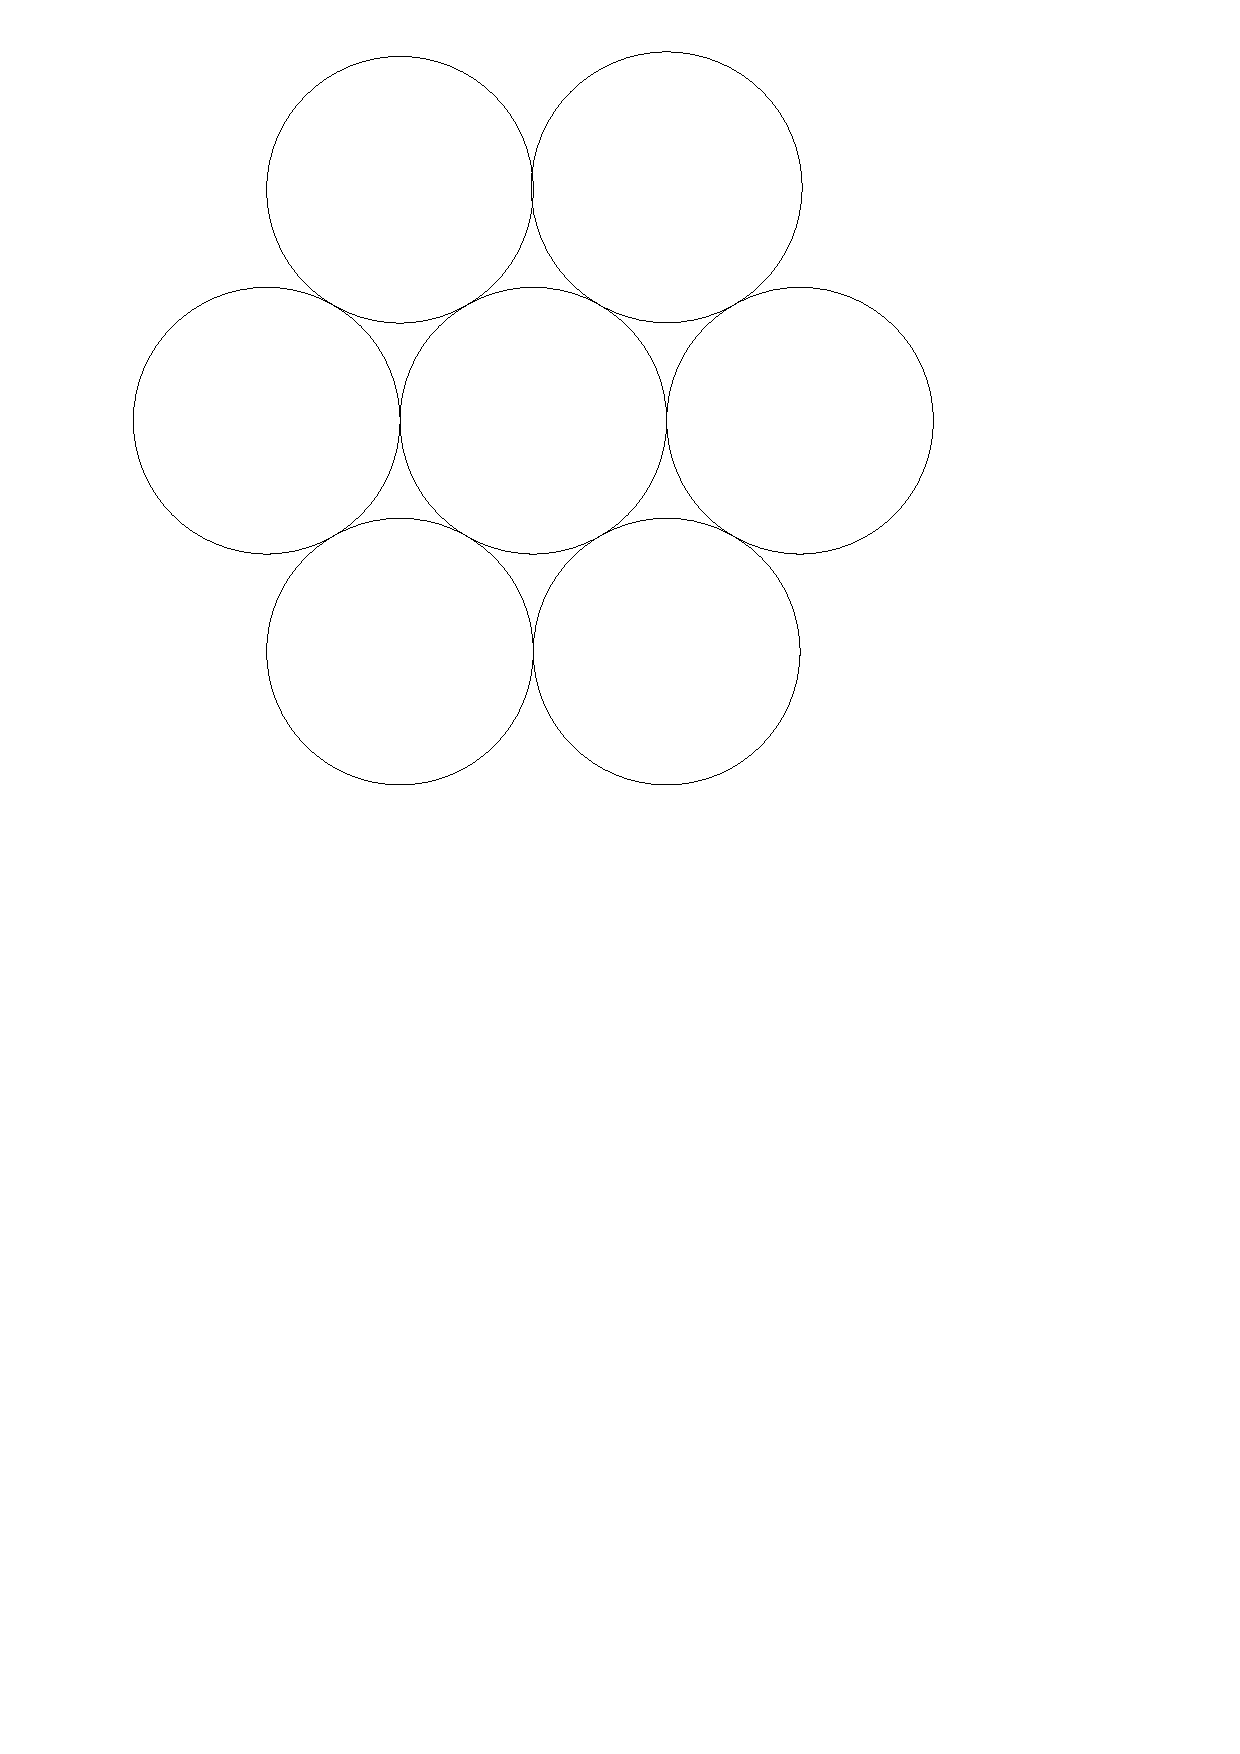
\includegraphics{graphics/7ballLocked.pdf}
\caption{A locked 7 ball configuration}
\end{center} 
\end{figure}
\newpage